\documentclass[12pt,a4paper]{report}
\usepackage[utf8]{inputenc}
\usepackage[T1]{fontenc}
\usepackage[french]{babel}
\usepackage{lmodern}
\usepackage{geometry}
\usepackage{graphicx}
\usepackage{xcolor}
\usepackage{array}
\usepackage{longtable}
\usepackage{booktabs}
\usepackage{enumitem}
\usepackage{fancyhdr}
\usepackage{hyperref}
\usepackage{listings}
\usepackage{caption}
\usepackage{float}
\usepackage{titlesec}

\geometry{margin=2.4cm}
\definecolor{MonBlue}{HTML}{1976D2}
\definecolor{MonNavy}{HTML}{18212F}
\definecolor{MonRed}{HTML}{C8323D}
\definecolor{MonText}{HTML}{263244}

\hypersetup{
  colorlinks=true,
  linkcolor=MonBlue,
  urlcolor=MonRed,
  pdftitle={Rapport PFE - Mon PF App},
  pdfauthor={HAJJI Yassmine}
}

\graphicspath{
  {../assets/}
  {../../tutorial/assets/source/}
  {../../tutorial/assets/screenshots/}
}

\pagestyle{fancy}
\fancyhf{}
\lhead{\small Mon PF App}
\rhead{\small HAJJI Yassmine -- BTS DAI}
\cfoot{\small \thepage}
\setlength{\headheight}{14pt}

\titleformat{\chapter}
  {\normalfont\Huge\bfseries\color{MonBlue}}
  {\thechapter}{1em}{}
\titleformat{\section}
  {\normalfont\Large\bfseries\color{MonNavy}}
  {\thesection}{0.8em}{}
\titleformat{\subsection}
  {\normalfont\large\bfseries\color{MonText}}
  {\thesubsection}{0.6em}{}

\setlist[itemize]{topsep=4pt,itemsep=3pt}
\setlist[enumerate]{topsep=4pt,itemsep=3pt}
\renewcommand{\arraystretch}{1.25}

\lstdefinestyle{monpf}{
  backgroundcolor=\color{black!92},
  basicstyle=\ttfamily\small\color{white},
  breaklines=true,
  frame=single,
  rulecolor=\color{black!20},
  xleftmargin=4pt,
  xrightmargin=4pt
}

\newcommand{\field}[2]{\textbf{#1} & #2\\}

\begin{document}

\hypersetup{pageanchor=false}
\begin{titlepage}
  \centering
  {\small Royaume du Maroc\\}
  {\small Ministère de l'Éducation Nationale, du Préscolaire et des Sports\\}
  {\small Académie Régionale de l'Éducation et de la Formation Drâa-Tafilalet\\}
  {\small Direction Provinciale de Ouarzazate\\[0.8cm]}

  
\includegraphics[width=3.2cm]{cover_image_1.png}\\[0.8cm]

  {\Huge\bfseries Rapport de Projet de Fin d'Études\\[0.35cm]}
  {\Large Deuxième année BTS\\}
  {\Large Développement des Applications Informatiques\\[1.0cm]}

  {\Large\bfseries\color{MonRed}
  Conception et réalisation d'une application mobile de gestion des commandes d'un restaurant\\[0.6cm]}
  {\Huge\bfseries Mon PF App\\[1.0cm]}

  \begin{tabular}{>{\bfseries}p{4cm}p{9cm}}
    Projet & Mon PF App\\
    Réalisé par & HAJJI Yassmine\\
    Établissement & Lycée Qualifiant Technique Ibn Al-Haitam\\
    Formation & BTS Développement des Applications Informatiques\\
    Encadrement & Encadrant pédagogique : Abdellah Ait Omar\\
    Année de formation & 2024 -- 2026\\
  \end{tabular}
\end{titlepage}
\hypersetup{pageanchor=true}

\pagenumbering{roman}

\begingroup
\pagestyle{empty}
\makeatletter
\let\ps@plain\ps@empty
\makeatother
\tableofcontents
\thispagestyle{empty}
\clearpage
\endgroup
\pagestyle{fancy}

\chapter*{Remerciements}
\addcontentsline{toc}{chapter}{Remerciements}
\vspace*{0.7cm}
Avant de présenter ce travail, je tiens à exprimer ma profonde gratitude à l'équipe pédagogique du BTS Développement des Applications Informatiques du Lycée Qualifiant Technique Ibn Al-Haitam. Les enseignements reçus durant cette formation m'ont permis d'acquérir une méthode de travail, une vision technique et une discipline nécessaires pour mener un projet informatique complet.

Je remercie également les enseignants et encadrants qui m'ont accompagnée dans l'apprentissage de l'analyse, de la conception, de la programmation, des bases de données et de la documentation technique. Leurs remarques et leurs conseils ont contribué à améliorer la qualité de ce projet et à mieux organiser les différentes étapes de réalisation.

Mes remerciements s'adressent aussi à toutes les personnes qui ont participé aux tests de l'application \textbf{Mon PF App}, que ce soit par leurs observations, leurs questions ou leurs retours d'utilisation. Ces retours ont aidé à rendre l'interface plus claire, les parcours plus simples et la démonstration plus cohérente.

Je remercie enfin ma famille pour son soutien, sa patience et ses encouragements pendant toute la période de préparation de ce projet de fin d'études. Ce travail représente une étape importante dans mon parcours de formation, car il m'a permis d'appliquer les connaissances acquises à une situation concrète : la gestion numérique des commandes d'un restaurant.

Ce projet m'a donné l'occasion de relier plusieurs compétences : développement mobile avec Flutter, création d'une API Laravel, conception de base de données, sécurité des rôles, tests, génération d'un APK Android et rédaction d'une documentation académique. Il constitue donc une synthèse pratique des apprentissages réalisés durant la formation.

\vfill
\begin{flushright}
\textit{HAJJI Yassmine}
\end{flushright}

\chapter*{Résumé}
\addcontentsline{toc}{chapter}{Résumé}
\vspace*{0.7cm}
\textbf{Mon PF App} est une application mobile et multi-plateforme destinée à la gestion des commandes d'un restaurant. Le projet répond à un besoin fréquent dans le domaine de la restauration : simplifier la prise de commande, limiter les erreurs manuelles, organiser le suivi et faciliter la communication entre le client, le restaurant et le livreur.

L'application permet au client de consulter le menu, choisir des plats, gérer son panier, passer une commande et suivre l'état de cette commande. Elle propose également des espaces adaptés aux autres acteurs du système : l'administrateur peut consulter les statistiques et les commandes, le serveur peut suivre le traitement opérationnel, et le livreur peut consulter les livraisons disponibles et accepter une commande.

Sur le plan technique, la solution repose sur \textbf{Flutter} pour le développement de l'interface Android, Windows et Web, et sur \textbf{Laravel} pour la création de l'API REST. Les données de démonstration sont stockées dans une base SQLite, ce qui permet de lancer rapidement le projet sur une machine locale pendant la soutenance.

Le projet inclut plusieurs améliorations importantes : suppression du choix de rôle dans l'inscription publique, contrôle des rôles côté backend, stockage sécurisé du token côté application, configuration de l'URL API par environnement, support du lancement Web local avec CORS, tests backend et guide HTML interactif pour aider à l'installation et au dépannage.

Ce rapport présente le contexte du projet, les besoins fonctionnels et non fonctionnels, la modélisation UML, l'architecture technique, la réalisation du backend et du frontend, les tests, les difficultés rencontrées et les perspectives d'amélioration. La version livrée constitue une version \textbf{démo-prod}, adaptée à une présentation académique et suffisamment structurée pour montrer un flux complet de commande restaurant.

\vfill
\noindent\textbf{Mots-clés :} Flutter, Laravel, API REST, restaurant, commande, livraison, SQLite, Android, Windows, Web, PFE.

\phantomsection
\pagenumbering{arabic}

\chapter{Présentation}
\section{Fiche signalétique}
\begin{table}[H]
\centering
\caption{Fiche signalétique du projet}
\begin{tabular}{p{4cm}p{10cm}}
\toprule
\textbf{Élément} & \textbf{Description}\\
\midrule
\field{Projet}{Mon PF App}
\field{Sujet}{Application mobile de gestion des commandes d'un restaurant}
\field{Réalisé par}{HAJJI Yassmine}
\field{Formation}{BTS Développement des Applications Informatiques}
\field{Établissement}{Lycée Qualifiant Technique Ibn Al-Haitam}
\field{Cibles}{Android, Windows et Web pour la démonstration}
\field{Période}{Année de formation 2024 -- 2026}
\bottomrule
\end{tabular}
\end{table}

\section{Intérêt du sujet}
Le secteur de la restauration utilise de plus en plus les outils numériques pour recevoir les commandes, réduire les erreurs et améliorer la communication avec les clients. Une application de commande constitue donc un sujet pertinent pour un PFE, car elle combine interface mobile, base de données, API REST, sécurité et gestion des rôles.

Le projet mobilise plusieurs compétences de la formation :
\begin{itemize}
  \item analyse du besoin et rédaction du cahier de charge ;
  \item modélisation UML et conception de données ;
  \item développement mobile avec Flutter ;
  \item développement backend avec Laravel ;
  \item tests, build Android et documentation.
\end{itemize}

\section{Organisation du rapport}
La structure du rapport suit la logique académique observée dans les rapports de PFE fournis comme références : présentation, contexte et spécification générale, modélisation UML, architecture technique, réalisation, conclusion et perspectives.

\chapter{Contexte et spécification générale}
\section{Contexte du projet}
Dans un restaurant, la prise de commande peut devenir difficile lorsque plusieurs clients commandent en même temps. Les erreurs de saisie, les oublis de plats, les retards de préparation et le manque de suivi entraînent une mauvaise expérience client.

L'application proposée répond à ce contexte en centralisant le menu, le panier, les commandes et les statuts. Elle permet au client de voir ce qu'il commande, au restaurant de recevoir les commandes et au livreur de connaître les livraisons disponibles.

\section{Problématique}
\begin{quote}
Comment digitaliser le parcours de commande d'un restaurant afin de réduire les erreurs humaines, améliorer le suivi des commandes et fournir une interface simple aux clients, administrateurs, serveurs et livreurs ?
\end{quote}

\section{Objectifs du projet}
L'objectif général est de réaliser une application fonctionnelle et présentable pour une démonstration PFE, avec un backend local et des données persistantes.

Les objectifs spécifiques sont :
\begin{itemize}
  \item permettre aux clients de consulter le menu ;
  \item gérer un panier et calculer automatiquement le total ;
  \item passer une commande réelle via API ;
  \item suivre le statut d'une commande ;
  \item proposer un espace administrateur et serveur ;
  \item proposer un espace livreur ;
  \item sécuriser l'inscription publique en imposant le rôle client côté serveur ;
  \item fournir un guide de lancement pour Android, Windows et Web.
\end{itemize}

\section{Spécification fonctionnelle générale}
\begin{longtable}{p{4cm}p{10cm}}
\caption{Besoins fonctionnels par acteur}\\
\toprule
\textbf{Acteur} & \textbf{Fonctionnalités attendues}\\
\midrule
Client & Créer un compte, se connecter, consulter le menu, ajouter des plats au panier, passer une commande, suivre son état.\\
Administrateur & Voir les statistiques, consulter les commandes, gérer le menu, affecter un livreur, contrôler les rôles sensibles.\\
Serveur & Participer au traitement opérationnel des commandes côté restaurant.\\
Livreur & Voir les commandes disponibles, accepter une livraison et mettre à jour son avancement.\\
\bottomrule
\end{longtable}

\section{Besoins non fonctionnels}
\begin{itemize}
  \item \textbf{Sécurité :} authentification, token et contrôle d'accès par rôle ;
  \item \textbf{Simplicité :} interface claire pour faciliter la prise en main ;
  \item \textbf{Rapidité :} accès rapide au menu et au panier ;
  \item \textbf{Fiabilité :} données seedées et tests automatiques ;
  \item \textbf{Maintenabilité :} séparation frontend, backend et documentation.
\end{itemize}

\chapter{Modélisation UML}
\section{Présentation d'UML}
UML est un langage de modélisation utilisé pour représenter les acteurs, les cas d'utilisation, les classes, les relations et les scénarios d'un système. Dans ce projet, UML sert à clarifier le fonctionnement avant et pendant la réalisation.

\section{Diagrammes UML employés}
Les diagrammes retenus sont :
\begin{itemize}
  \item le diagramme de cas d'utilisation pour identifier les actions de chaque acteur ;
  \item le diagramme de classes pour représenter les entités principales ;
  \item le diagramme de séquence pour expliquer le passage d'une commande.
\end{itemize}

\section{Cas d'utilisation}
\begin{longtable}{p{4cm}p{10cm}}
\caption{Cas d'utilisation principaux}\\
\toprule
\textbf{Acteur} & \textbf{Cas d'utilisation}\\
\midrule
Client & S'inscrire, se connecter, consulter le menu, gérer le panier, valider une commande, suivre le statut.\\
Administrateur & Consulter le tableau de bord, voir les commandes, gérer le menu, affecter un livreur.\\
Serveur & Suivre les commandes côté restaurant, modifier certains statuts.\\
Livreur & Consulter la file de livraison, accepter une commande, marquer l'avancement.\\
\bottomrule
\end{longtable}

\section{Diagramme de classes du système}
Le modèle de données repose sur les entités \texttt{User}, \texttt{Restaurant}, \texttt{Category}, \texttt{MenuItem}, \texttt{Order} et \texttt{OrderItem}. Le client est relié aux commandes, une commande contient plusieurs lignes et chaque ligne référence un plat.

\begin{figure}[H]
  \centering
  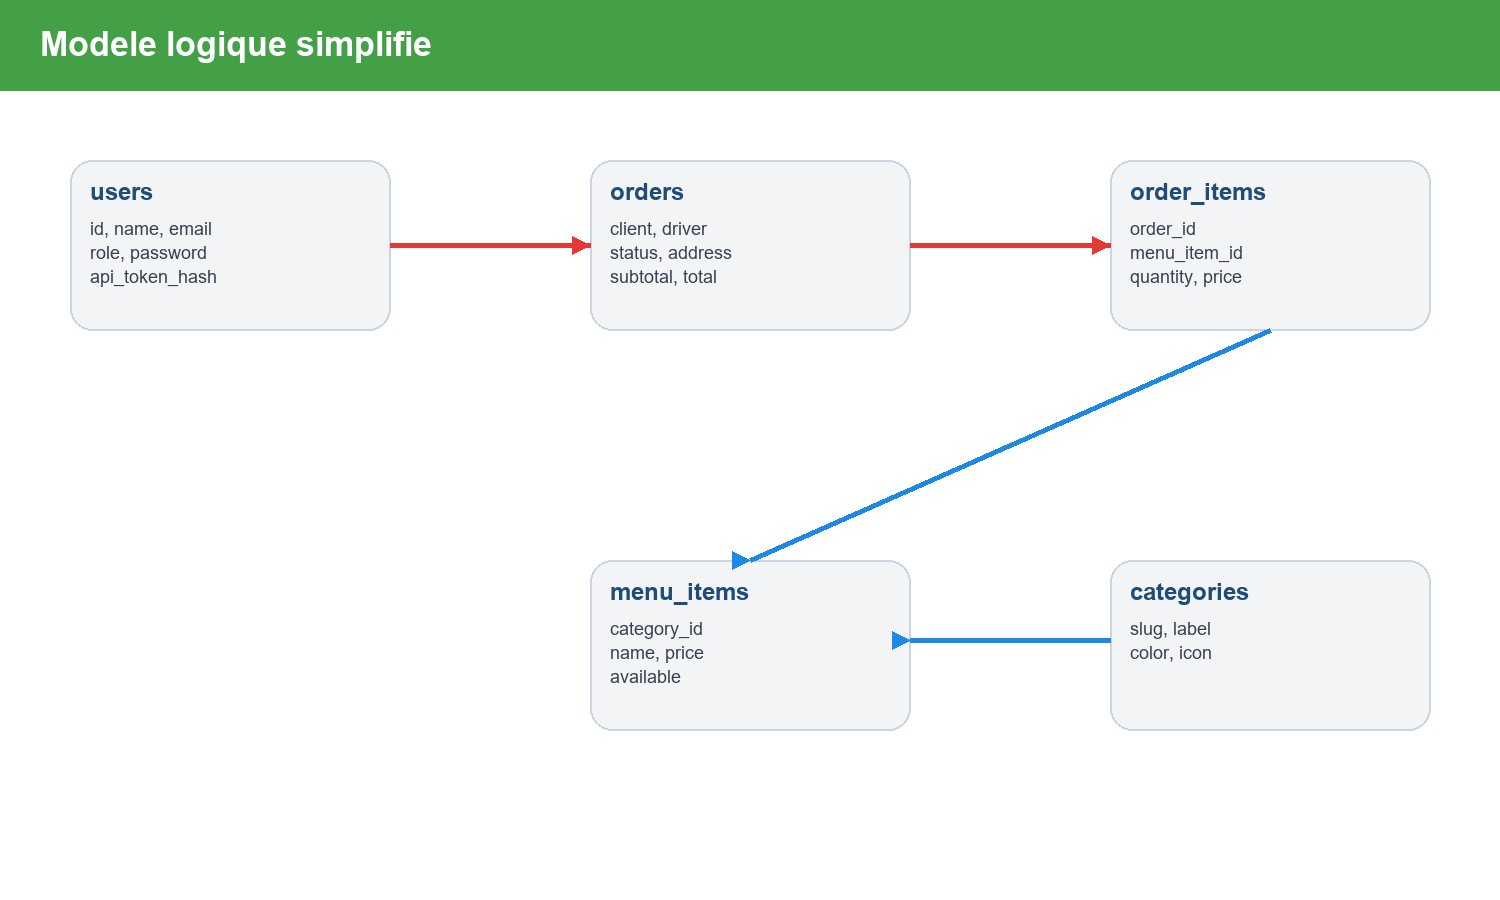
\includegraphics[width=\textwidth]{data_model_backend.png}
  \caption{Diagramme logique des classes et relations backend}
\end{figure}

\section{Diagramme de séquence : passer une commande}
Le scénario principal commence par la consultation du menu et se termine par la création d'une commande en base de données. Flutter prépare le panier, Laravel valide les données, puis l'API retourne la commande créée.

\begin{figure}[H]
  \centering
  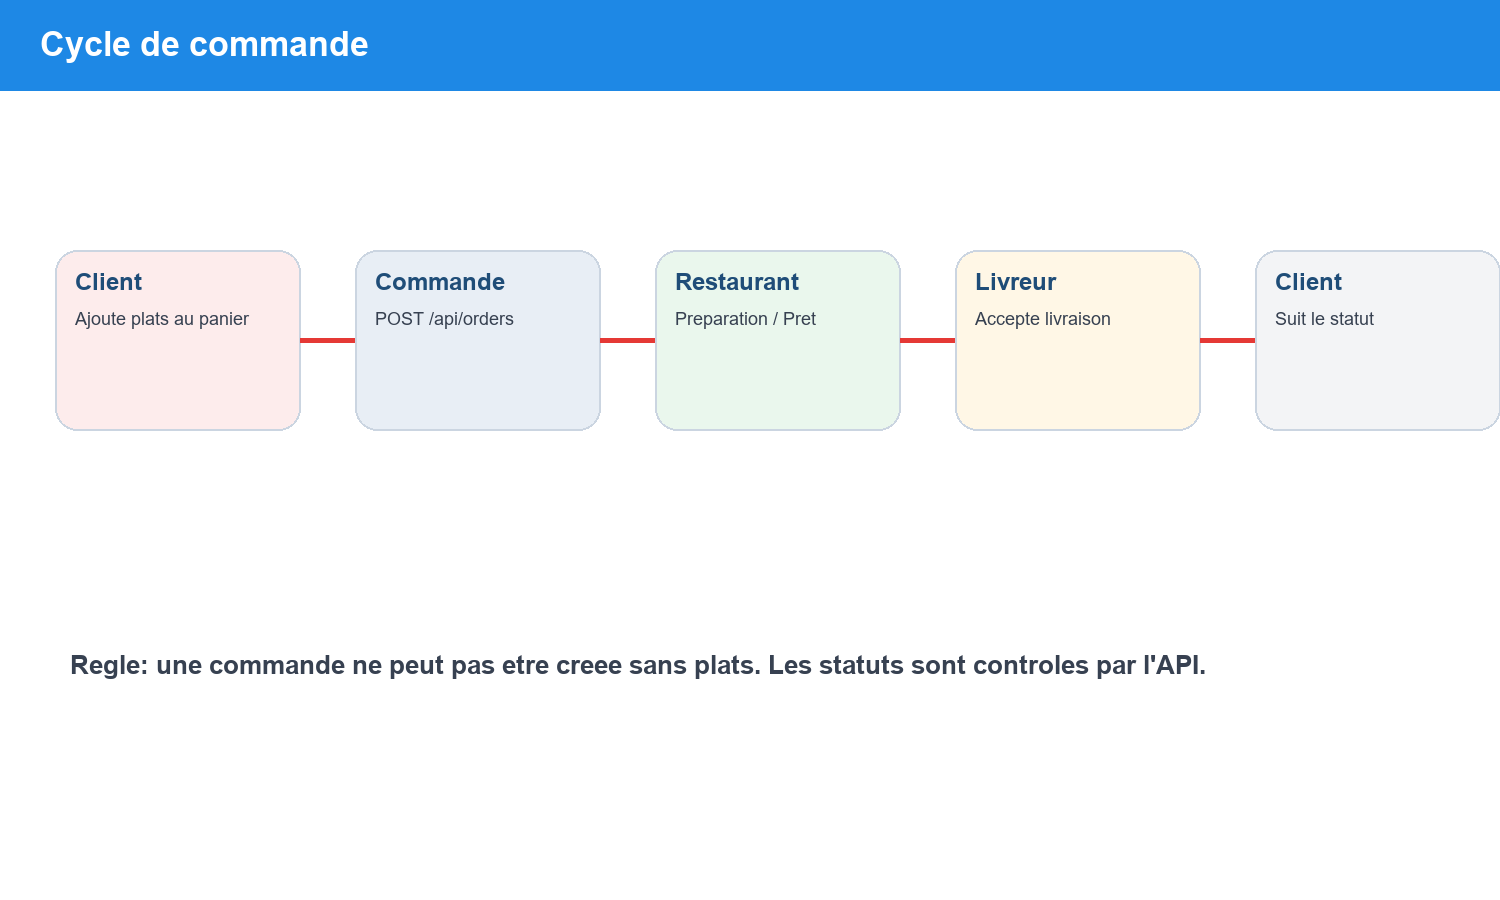
\includegraphics[width=\textwidth]{order_cycle.png}
  \caption{Séquence simplifiée du cycle de commande}
\end{figure}

\chapter{Architecture technique et technologies utilisées}
\section{Étude technique}
L'étude technique a pour objectif de choisir une architecture simple à lancer en soutenance, mais suffisamment structurée pour représenter une application réelle. Le choix s'est porté sur Flutter pour l'interface et Laravel pour le backend.

\begin{figure}[H]
  \centering
  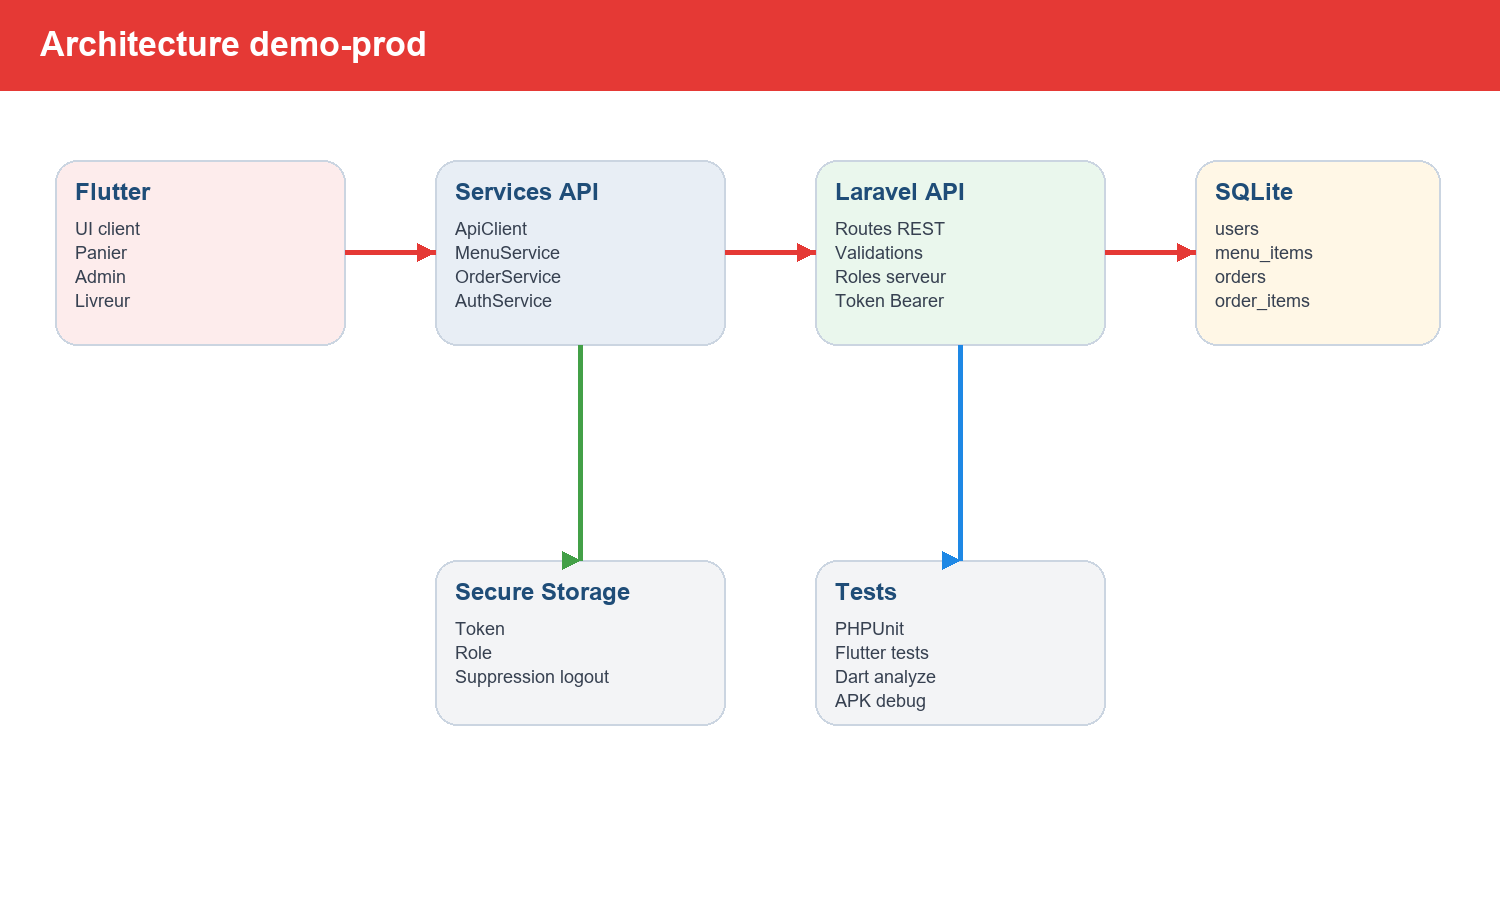
\includegraphics[width=\textwidth]{architecture_demo_prod.png}
  \caption{Vue d'ensemble de l'architecture démo-prod}
\end{figure}

\section{Critères de sélection}
Les critères utilisés pour choisir les technologies sont :
\begin{itemize}
  \item facilité de mise en place sur la machine de démonstration ;
  \item clarté du code pour un projet BTS ;
  \item compatibilité Android, Windows et Web ;
  \item possibilité de tests automatiques ;
  \item documentation et communauté disponibles.
\end{itemize}

\section{Langages de développement}
\begin{table}[H]
\centering
\caption{Langages utilisés}
\begin{tabular}{p{4cm}p{10cm}}
\toprule
\textbf{Langage} & \textbf{Utilisation}\\
\midrule
Dart & Développement de l'application Flutter.\\
PHP & Développement de l'API Laravel.\\
SQL & Définition et manipulation de la base SQLite.\\
HTML/CSS/JavaScript & Guide interactif local et assistant debug pour Yassmine.\\
\bottomrule
\end{tabular}
\end{table}

\section{Frameworks et outils}
\begin{longtable}{p{4cm}p{4cm}p{6cm}}
\caption{Choix techniques}\\
\toprule
\textbf{Couche} & \textbf{Technologie} & \textbf{Justification}\\
\midrule
Frontend & Flutter & Interface unique pour Android, Windows et Web.\\
Backend & Laravel 13 & Routes REST, validations, tests, structure MVC.\\
Base démo & SQLite & Démarrage rapide sans serveur de base externe.\\
Sécurité mobile & \texttt{flutter\_secure\_storage} & Stockage plus sûr du token local.\\
Tests backend & PHPUnit & Vérification automatique des flux API.\\
Documentation & LaTeX + HTML & Rapport académique et guide interactif.\\
\bottomrule
\end{longtable}

\section{Sécurité technique}
Les décisions de sécurité importantes sont :
\begin{itemize}
  \item le rôle n'est plus choisi depuis l'inscription publique ;
  \item le backend force le rôle \texttt{client} pour \texttt{/api/register} ;
  \item les routes sensibles sont protégées par middleware ;
  \item les tokens sont stockés côté Flutter avec \texttt{flutter\_secure\_storage} ;
  \item l'URL API est fournie par \texttt{API\_BASE\_URL} au lieu d'être codée en dur ;
  \item CORS est activé pour la démonstration Web locale.
\end{itemize}

\chapter{Réalisation}
\section{Architecture de l'application}
Le dépôt est organisé en trois zones principales :
\begin{itemize}
  \item \texttt{mon\_pfapp} : application Flutter ;
  \item \texttt{mon\_pfapi} : API Laravel ;
  \item \texttt{docs} : cahier de charge, rapports, tutoriels et guide HTML.
\end{itemize}

\section{Réalisation backend}
Le backend expose des endpoints REST pour authentifier les utilisateurs, récupérer le menu, créer des commandes et gérer les statuts.

\begin{longtable}{p{3cm}p{5cm}p{6cm}}
\caption{Endpoints API principaux}\\
\toprule
\textbf{Méthode} & \textbf{Endpoint} & \textbf{Rôle}\\
\midrule
GET & \texttt{/api/health} & Vérifier que l'API fonctionne.\\
GET & \texttt{/api/menu} & Récupérer le restaurant, les catégories et les plats.\\
POST & \texttt{/api/register} & Créer un compte client.\\
POST & \texttt{/api/login} & Authentifier et retourner un token.\\
GET & \texttt{/api/orders} & Lister les commandes selon le rôle.\\
POST & \texttt{/api/orders} & Créer une commande depuis le panier.\\
PATCH & \texttt{/api/orders/\{order\}/status} & Mettre à jour le statut.\\
GET & \texttt{/api/admin/stats} & Consulter les statistiques.\\
GET & \texttt{/api/driver/orders} & Voir la file de livraison.\\
\bottomrule
\end{longtable}

\section{Réalisation frontend}
L'application Flutter contient des écrans pour l'authentification, l'accueil, le menu, le panier, le suivi, le profil, l'espace livreur et l'espace admin. Des images de plats et un logo personnalisé remplacent l'interface Flutter par défaut.

\clearpage
\begin{figure}[H]
  \centering
  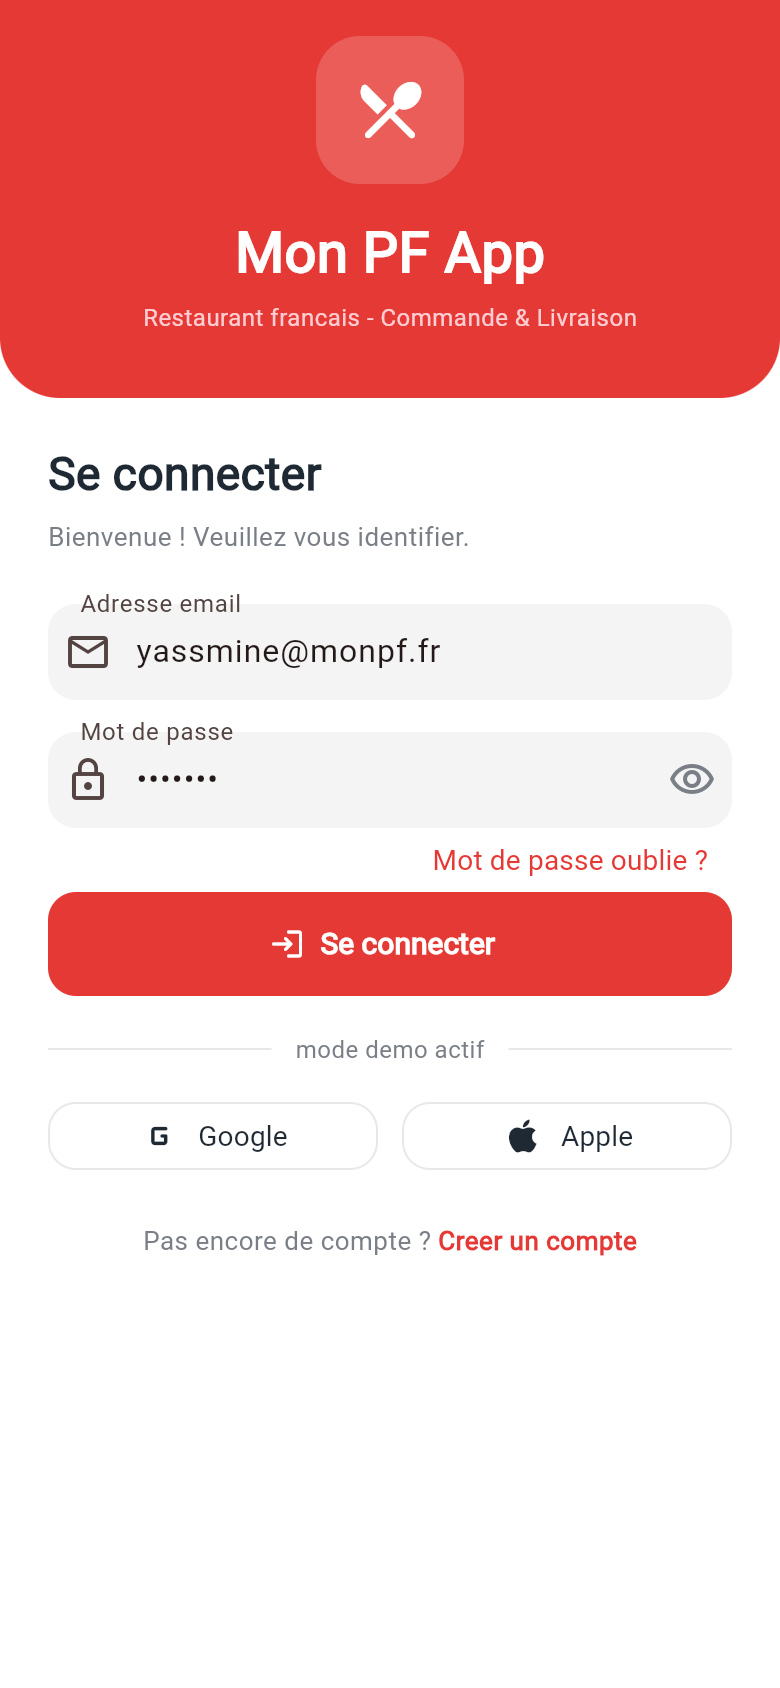
\includegraphics[height=0.70\textheight,keepaspectratio]{01-login.png}
  \caption{Écran de connexion}
\end{figure}
\clearpage

\begin{figure}[H]
  \centering
  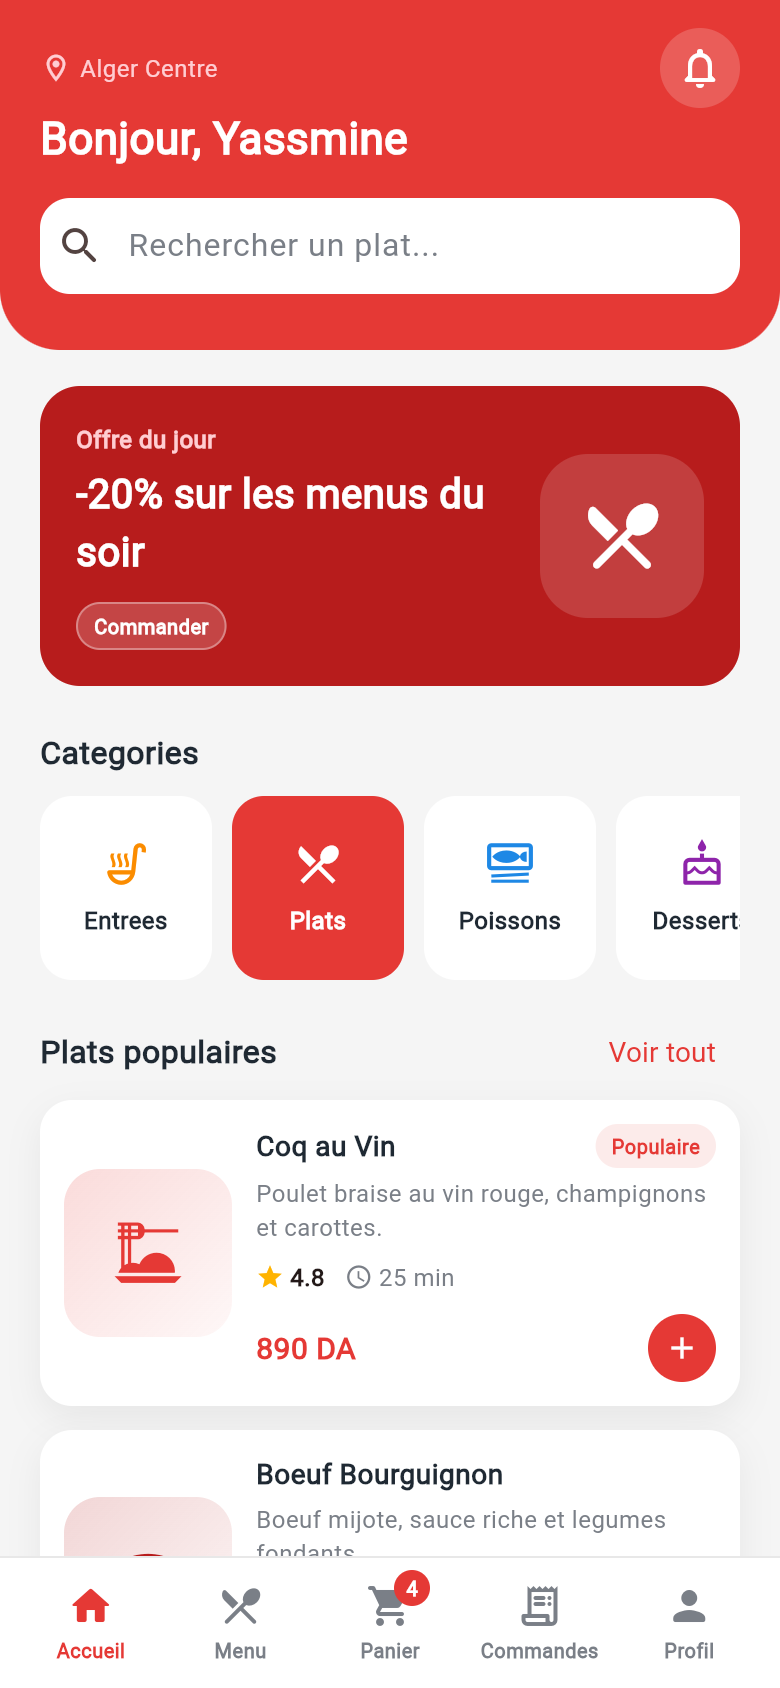
\includegraphics[height=0.70\textheight,keepaspectratio]{02-home.png}
  \caption{Écran d'accueil client}
\end{figure}
\clearpage

\begin{figure}[H]
  \centering
  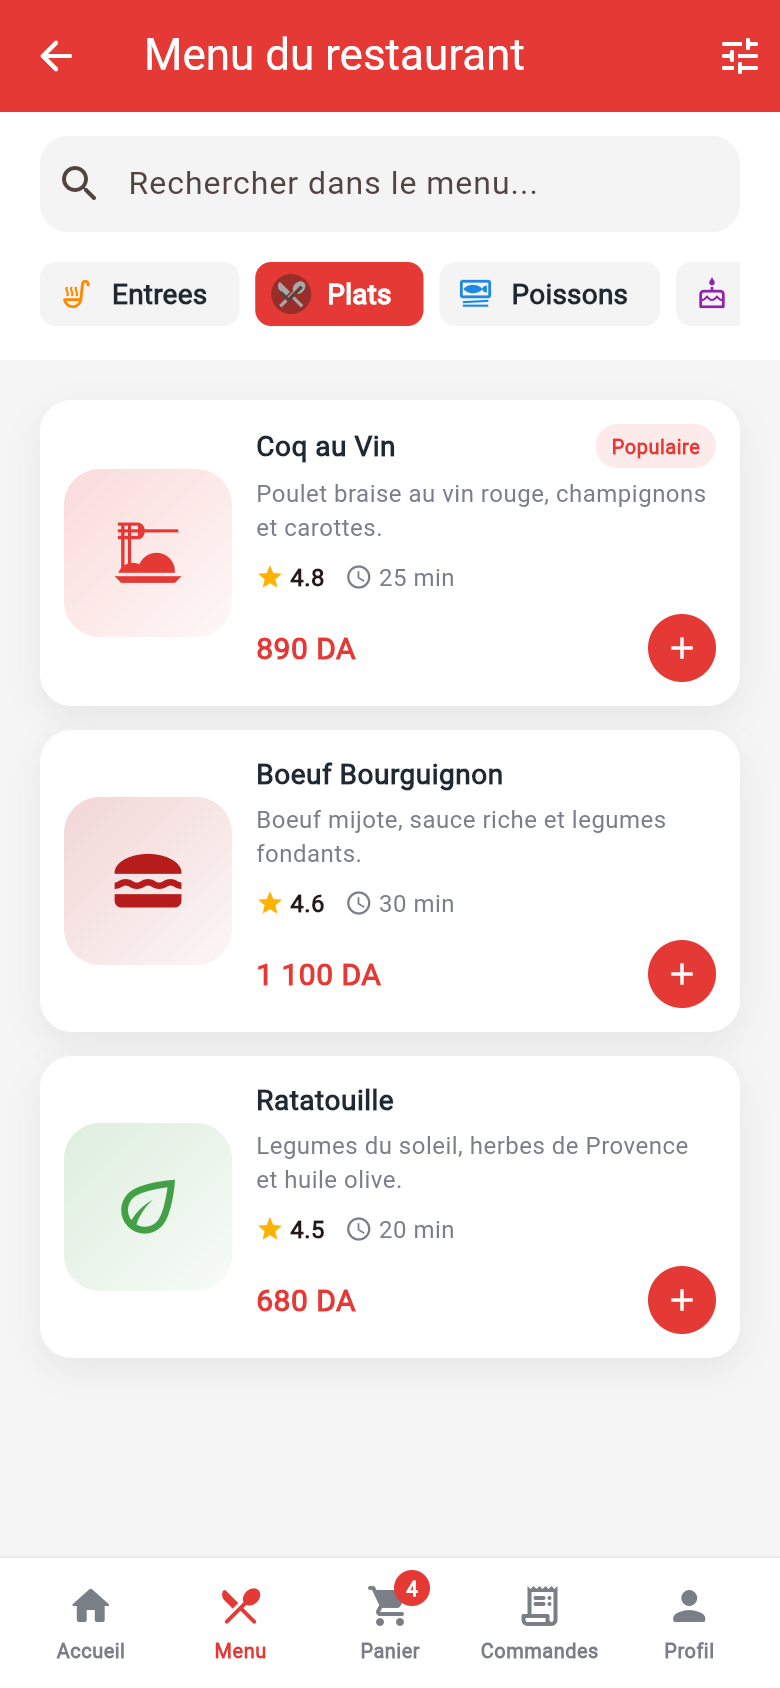
\includegraphics[height=0.70\textheight,keepaspectratio]{03-menu.png}
  \caption{Écran du menu et des plats}
\end{figure}
\clearpage

\begin{figure}[H]
  \centering
  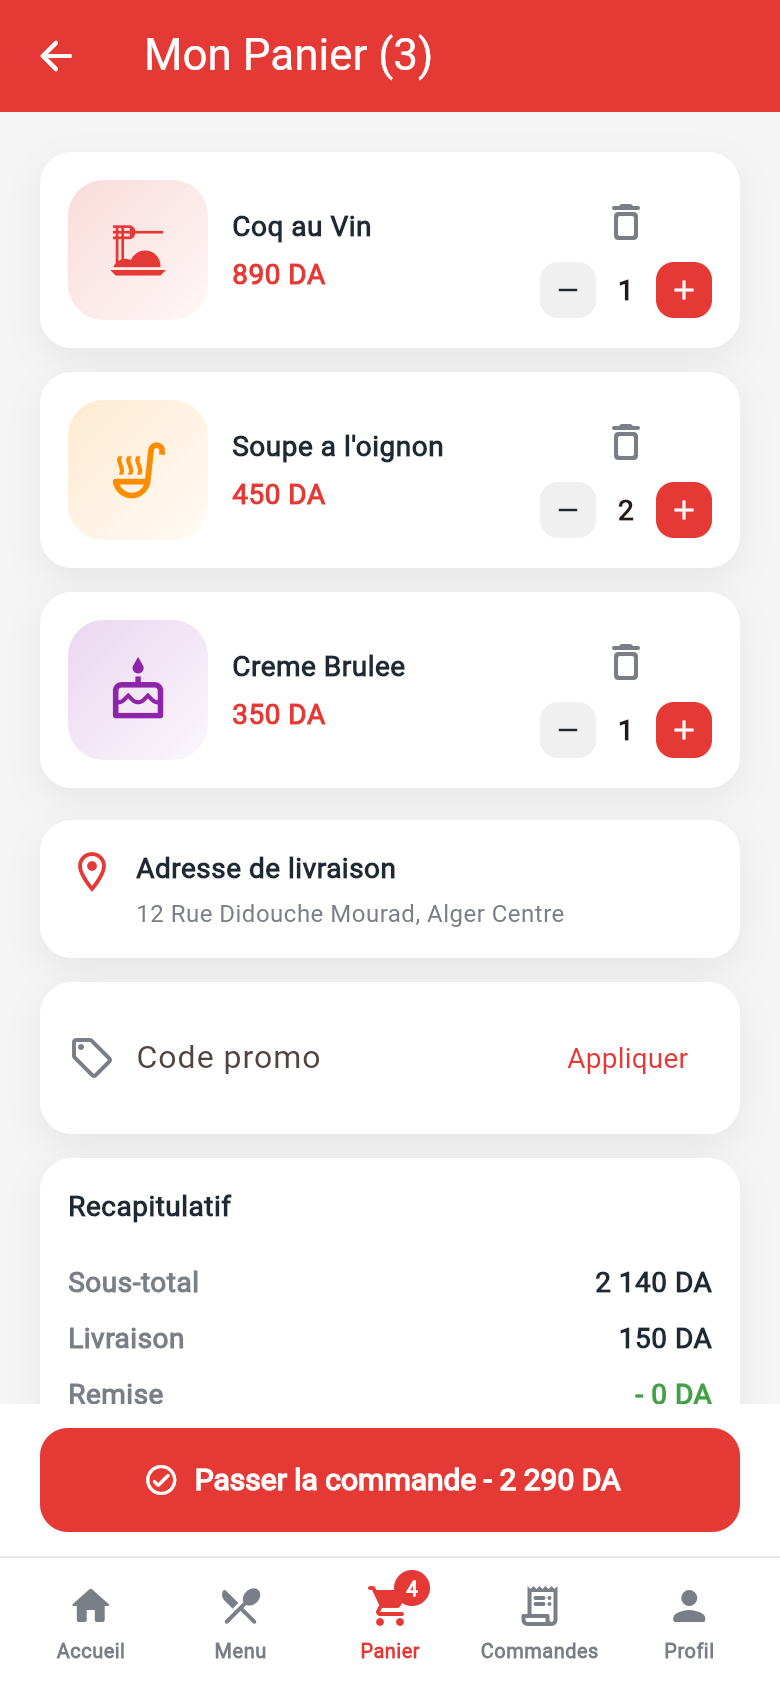
\includegraphics[height=0.70\textheight,keepaspectratio]{04-cart.png}
  \caption{Écran du panier}
\end{figure}
\clearpage

\begin{figure}[H]
  \centering
  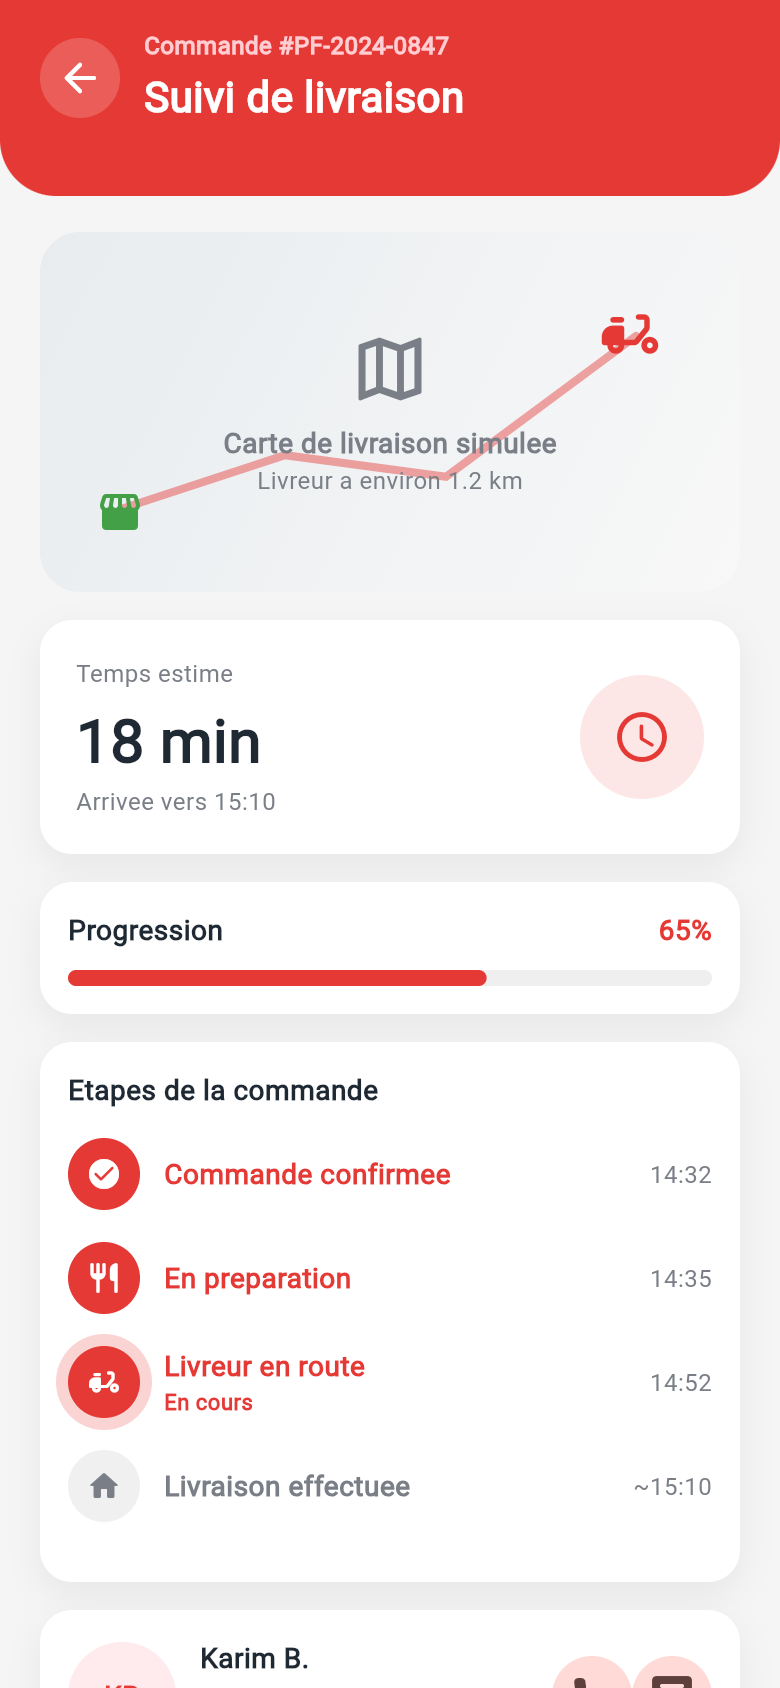
\includegraphics[height=0.70\textheight,keepaspectratio]{05-tracking.png}
  \caption{Écran de suivi des commandes}
\end{figure}
\clearpage

\begin{figure}[H]
  \centering
  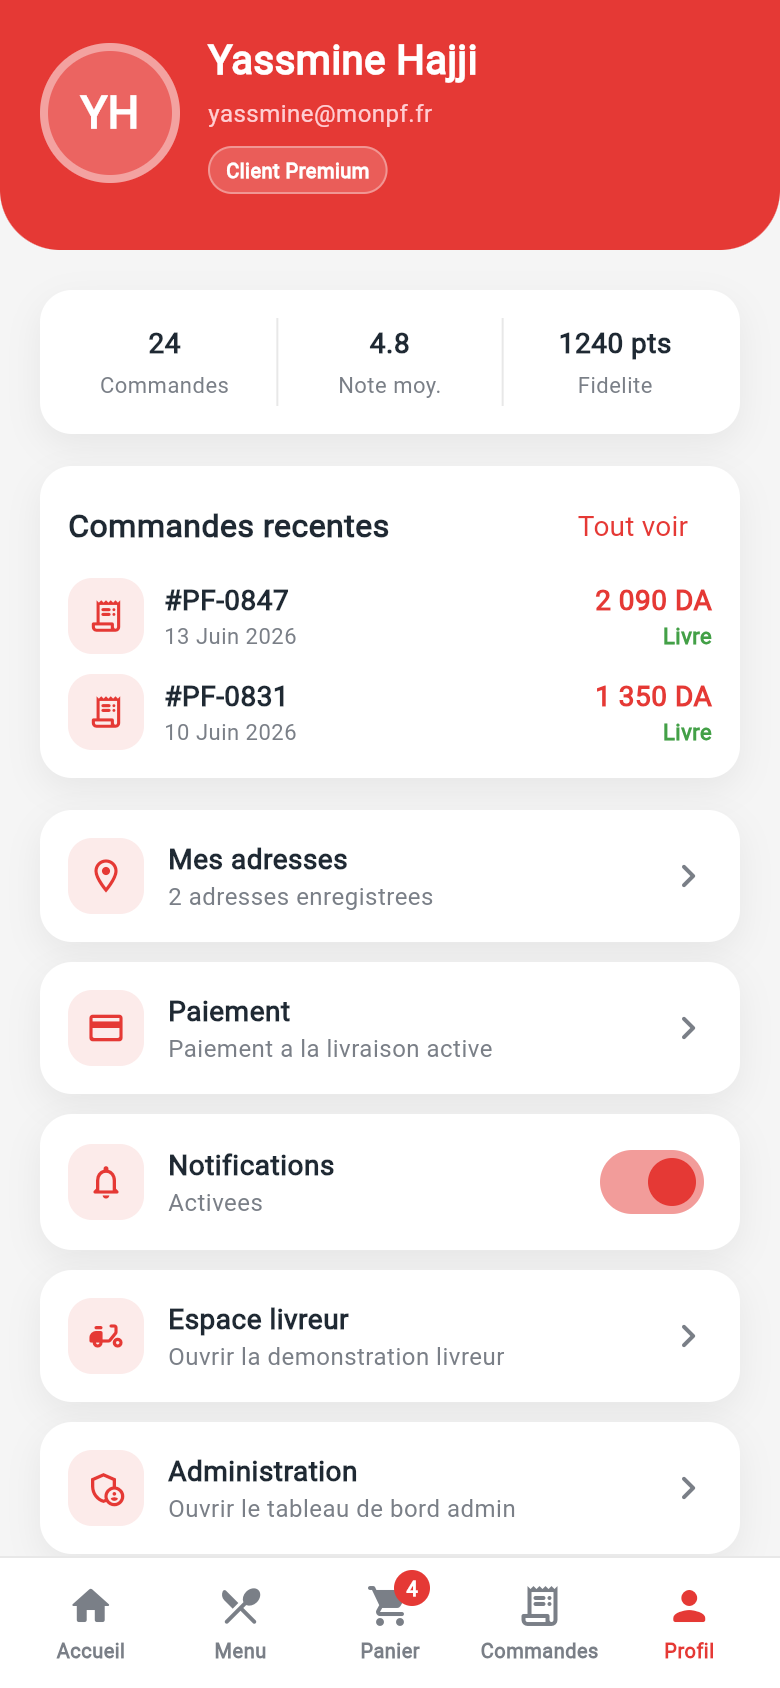
\includegraphics[height=0.70\textheight,keepaspectratio]{06-profile.png}
  \caption{Écran du profil client}
\end{figure}
\clearpage

\begin{figure}[H]
  \centering
  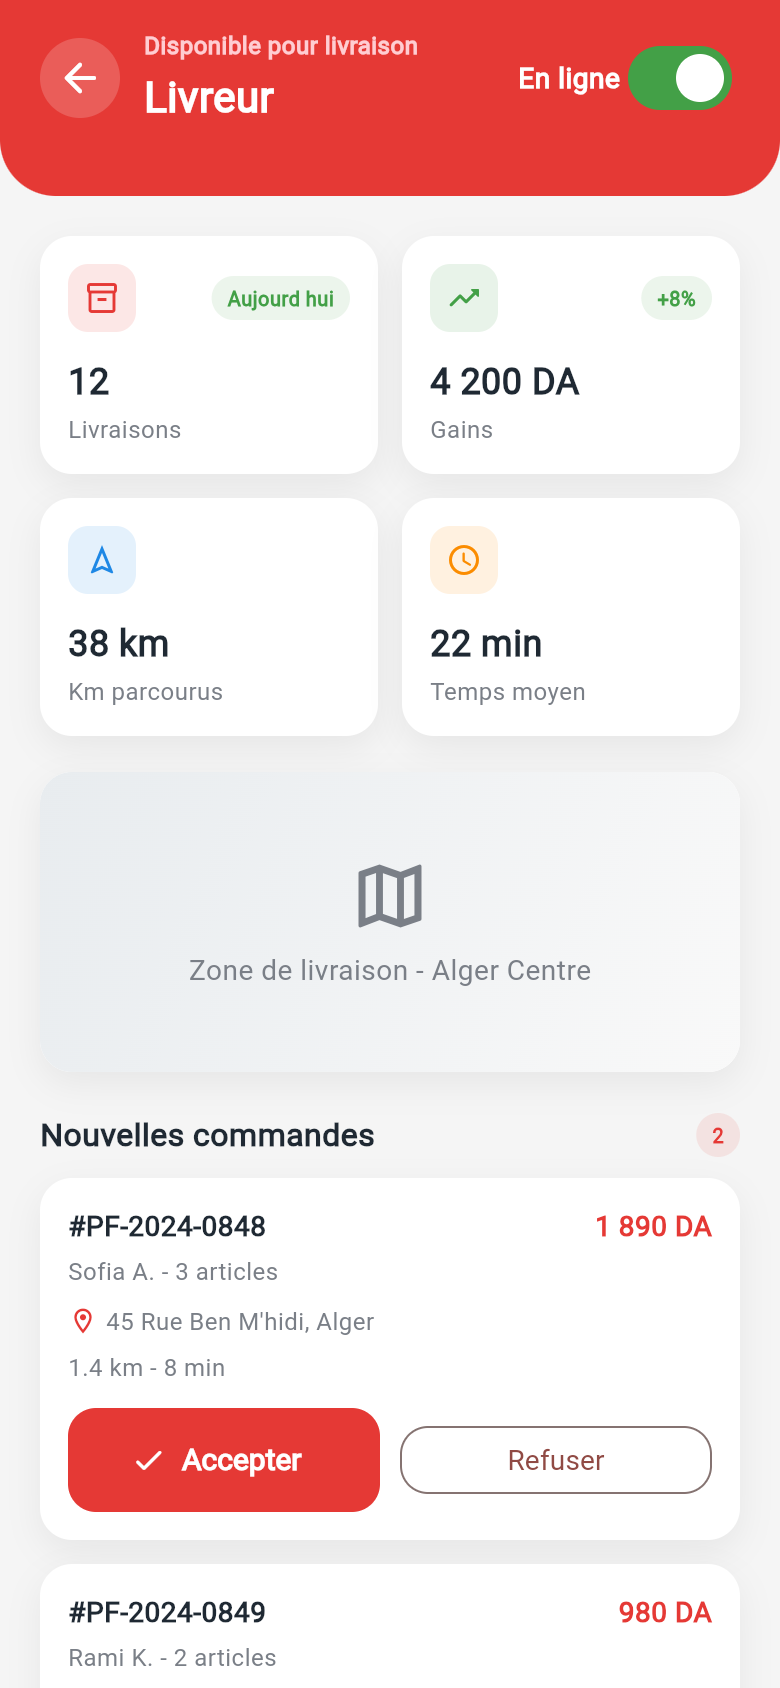
\includegraphics[height=0.70\textheight,keepaspectratio]{07-driver.png}
  \caption{Écran livreur}
\end{figure}
\clearpage

\begin{figure}[H]
  \centering
  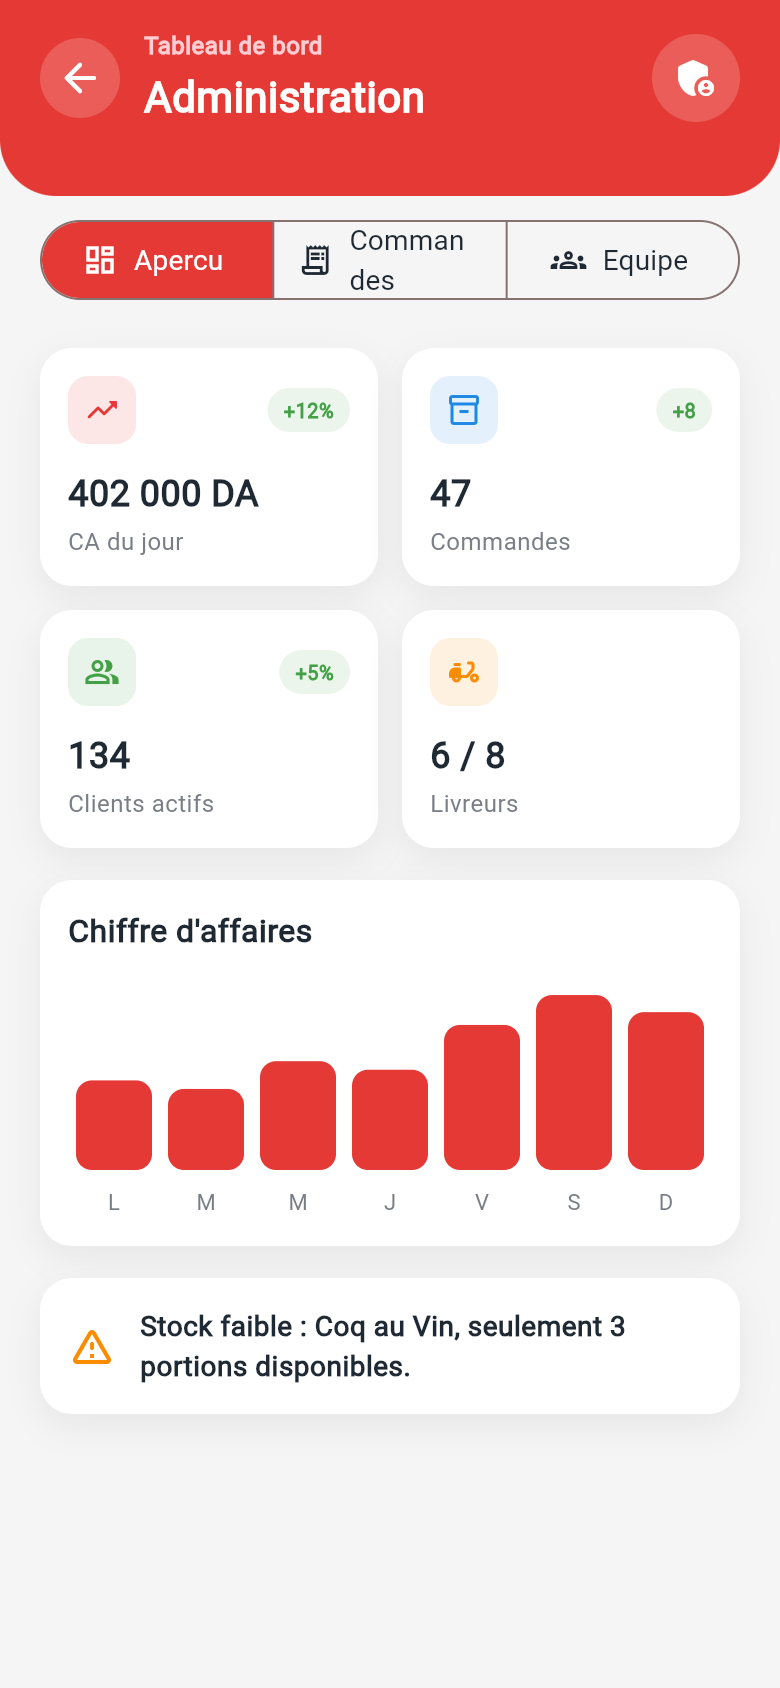
\includegraphics[height=0.70\textheight,keepaspectratio]{08-admin.png}
  \caption{Écran administrateur}
\end{figure}

\section{Guide interactif et assistant debug}
Un guide HTML local a été ajouté dans \texttt{docs/yassmine-guide/index.html}. Il sert de support pratique pour Yassmine : lancement Android, Windows, Web, utilisation de l'application, erreurs fréquentes et assistant debug basé sur Gemini API.

L'assistant ne contient aucune clé API dans le code source. La clé Gemini est saisie dans le navigateur uniquement au moment de l'utilisation. Si aucune clé n'est fournie, une base locale de solutions répond aux erreurs courantes.

\section{Structure détaillée du frontend Flutter}
La structure Flutter a été organisée pour séparer les responsabilités. Cette séparation facilite la lecture du code, les tests et les futures améliorations.

\begin{longtable}{p{5cm}p{9cm}}
\caption{Organisation du code Flutter}\\
\toprule
\textbf{Dossier ou fichier} & \textbf{Rôle dans l'application}\\
\midrule
\nolinkurl{lib/app/mon_pf_app.dart} & Point central de l'application : thème, navigation, état utilisateur, panier et chargement des données.\\
\nolinkurl{lib/core/config/api_config.dart} & Configuration du mode démo et de l'URL API via \texttt{dart-define}.\\
\nolinkurl{lib/core/storage/secure_token_store.dart} & Stockage sécurisé du token d'authentification.\\
\nolinkurl{lib/data/api_client.dart} & Client HTTP commun : headers, token, timeout et messages d'erreur.\\
\nolinkurl{lib/features/auth/} & Écrans et services de connexion, inscription et déconnexion.\\
\nolinkurl{lib/features/client/} & Écrans client : accueil, menu, panier, suivi et profil.\\
\nolinkurl{lib/features/admin/} & Écrans administrateur et serveur : statistiques, commandes et menu.\\
\nolinkurl{lib/features/driver/} & Écrans livreur : file de livraison et acceptation.\\
\nolinkurl{lib/shared/widgets/} & Composants réutilisables : cartes, boutons, navigation et visuels.\\
\bottomrule
\end{longtable}

\section{Structure détaillée du backend Laravel}
Le backend Laravel suit une organisation MVC. Les routes reçoivent les requêtes HTTP, les contrôleurs appliquent les règles métier, les modèles manipulent les données et les migrations définissent le schéma.

\begin{longtable}{p{5cm}p{9cm}}
\caption{Organisation du backend Laravel}\\
\toprule
\textbf{Dossier ou fichier} & \textbf{Rôle}\\
\midrule
\nolinkurl{routes/api.php} & Déclare les endpoints REST publics et protégés.\\
\nolinkurl{app/Http/Controllers/Api/AuthController.php} & Gère l'inscription, la connexion et la déconnexion.\\
\nolinkurl{app/Http/Controllers/Api/MenuController.php} & Fournit le catalogue restaurant et les actions de gestion menu.\\
\nolinkurl{app/Http/Controllers/Api/OrderController.php} & Gère la création, la consultation, les statuts et l'affectation des commandes.\\
\nolinkurl{app/Http/Middleware/TokenAuth.php} & Vérifie le token Bearer et les rôles autorisés.\\
\nolinkurl{database/migrations/} & Définit les tables de la base SQLite.\\
\nolinkurl{database/seeders/DatabaseSeeder.php} & Crée les comptes de démonstration, le restaurant, les catégories et les plats.\\
\nolinkurl{tests/Feature/ApiFlowTest.php} & Vérifie les flux API critiques.\\
\bottomrule
\end{longtable}

\section{Description des interfaces graphiques}
\begin{longtable}{p{4cm}p{10cm}}
\caption{Écrans principaux de l'application}\\
\toprule
\textbf{Écran} & \textbf{Description}\\
\midrule
Connexion & Permet à un utilisateur existant d'accéder à son espace selon son rôle.\\
Inscription & Crée un compte client. Le rôle n'est pas choisi dans l'interface publique.\\
Accueil client & Présente l'identité visuelle du restaurant et l'accès rapide au menu.\\
Menu & Affiche les catégories et les plats avec images, prix et ajout au panier.\\
Panier & Récapitule les plats, quantités, sous-totaux et total général.\\
Suivi & Affiche les commandes du client et leurs statuts.\\
Dashboard admin & Montre les statistiques utiles et la liste des commandes.\\
Espace livreur & Présente les commandes disponibles pour livraison et l'action d'acceptation.\\
\bottomrule
\end{longtable}

\section{Gestion des rôles}
Le système distingue quatre rôles : client, administrateur, serveur et livreur. Cette séparation répond à une règle importante : chaque utilisateur doit uniquement accéder aux actions qui correspondent à son métier.

\begin{longtable}{p{4cm}p{5cm}p{5cm}}
\caption{Contrôle d'accès par rôle}\\
\toprule
\textbf{Action} & \textbf{Rôles autorisés} & \textbf{Protection}\\
\midrule
Consulter le menu & Public & Route publique.\\
Créer une commande & Client connecté & Middleware token.\\
Lister toutes les commandes & Admin, serveur & Middleware rôle.\\
Modifier le statut & Admin, serveur, livreur selon cas & Middleware + validation métier.\\
Voir la file livreur & Admin, livreur & Middleware rôle.\\
Créer un administrateur & Non public & Action non exposée à l'inscription.\\
\bottomrule
\end{longtable}

\section{Algorithmes et règles métier}
\subsection{Calcul du total du panier}
\begin{lstlisting}[style=monpf,caption={Principe du calcul de total}]
total = 0
pour chaque ligne du panier:
    total = total + (prix_unitaire * quantite)
\end{lstlisting}

\subsection{Création d'une commande}
\begin{enumerate}
  \item Flutter vérifie que le panier n'est pas vide ;
  \item le panier est transformé en JSON ;
  \item Laravel vérifie l'utilisateur connecté ;
  \item Laravel valide les plats et les quantités ;
  \item Laravel crée la commande et ses lignes ;
  \item Flutter affiche le suivi de commande.
\end{enumerate}

\section{Tests et validation}
\begin{longtable}{p{4cm}p{5cm}p{5cm}}
\caption{Tests réalisés}\\
\toprule
\textbf{Zone} & \textbf{Commande} & \textbf{Objectif}\\
\midrule
Backend & \texttt{artisan test} & Tester menu, login, inscription client et commande.\\
Flutter & \texttt{flutter test} & Tester les flux auth/navigation.\\
Dart & \texttt{dart analyze} & Détecter les erreurs statiques.\\
Android & \texttt{flutter build apk} & Produire un APK installable.\\
LaTeX & \texttt{pdflatex} & Générer le rapport académique.\\
\bottomrule
\end{longtable}

\section{Mise en service locale}
\begin{lstlisting}[style=monpf,caption={Démarrer Laravel}]
cd C:\Users\LOQ\Documents\yassmin pfe\mon_pfapi
..\tools\runtime\php-8.4.22\php.exe artisan migrate:fresh --seed
..\tools\runtime\php-8.4.22\php.exe artisan serve --host=0.0.0.0 --port=8000
\end{lstlisting}

\begin{lstlisting}[style=monpf,caption={Lancer Flutter Windows}]
cd C:\Users\LOQ\Documents\yassmin pfe\mon_pfapp
flutter run -d windows --dart-define=DEMO_MODE=false --dart-define=API_BASE_URL=http://127.0.0.1:8000/api
\end{lstlisting}

\begin{lstlisting}[style=monpf,caption={Lancer Flutter Web}]
flutter run -d chrome --web-port=5600 --dart-define=DEMO_MODE=false --dart-define=API_BASE_URL=http://127.0.0.1:8000/api
\end{lstlisting}

\begin{lstlisting}[style=monpf,caption={Lancer Flutter Android réel}]
flutter run -d <device-id> --dart-define=DEMO_MODE=false --dart-define=API_BASE_URL=http://ADRESSE_IP_PC:8000/api
\end{lstlisting}

\section{Scénario de démonstration}
Le scénario recommandé pour la soutenance permet de montrer rapidement toute la chaîne fonctionnelle :
\begin{enumerate}
  \item démarrer l'API Laravel et tester \texttt{/api/health} ;
  \item lancer Flutter sur Android, Windows ou Web ;
  \item se connecter avec le compte client \texttt{yassmine@monpf.fr} ;
  \item consulter le menu et ajouter plusieurs plats au panier ;
  \item valider la commande et afficher le suivi ;
  \item se connecter avec le compte administrateur ;
  \item montrer les statistiques et les commandes ;
  \item se connecter avec le compte livreur ;
  \item accepter une commande disponible ;
  \item conclure en expliquant l'architecture Flutter + Laravel.
\end{enumerate}

\section{Guide de dépannage intégré}
Le guide HTML contient un assistant qui aide Yassmine à comprendre les erreurs d'installation. Il ne remplace pas la documentation technique, mais il donne une explication guidée : signification de l'erreur, cause probable dans le projet, solution pas à pas et commande de vérification.

Les erreurs couvertes localement sont notamment :
\begin{itemize}
  \item Android ne détecte pas le téléphone ;
  \item l'application Android n'arrive pas à joindre l'API ;
  \item Windows demande le fichier \texttt{atlstr.h} ;
  \item Web bloque les requêtes à cause de CORS ;
  \item Laravel n'est pas lancé ou le port 8000 est indisponible.
\end{itemize}

\chapter{Conclusion}
\section{Bilan}
Mon PF App répond au cœur du cahier de charge : authentification, menu, panier, commande, suivi, rôles et livraison. La version obtenue est adaptée à une soutenance PFE car elle présente une interface moderne, un backend fonctionnel, des données locales seedées, des tests et une documentation complète.

Le projet a permis de mettre en pratique les compétences de la formation BTS DAI : analyse, conception, base de données, développement mobile, API REST, sécurité, tests, documentation et mise en service.

\section{Difficultés rencontrées}
\begin{longtable}{p{4cm}p{5cm}p{5cm}}
\caption{Difficultés et solutions}\\
\toprule
\textbf{Difficulté} & \textbf{Cause} & \textbf{Solution}\\
\midrule
API locale sur téléphone & \texttt{127.0.0.1} pointe vers le téléphone & Utiliser l'IP Wi-Fi du PC.\\
Web et CORS & Origines différentes entre Chrome et Laravel & Ajouter \texttt{HandleCors} et \texttt{config/cors.php}.\\
Sécurité des rôles & Rôle sensible exposé à l'inscription & Imposer le rôle côté serveur.\\
Stockage token & Stockage simple insuffisant & Utiliser \texttt{flutter\_secure\_storage}.\\
Windows ATL & Composant Visual Studio absent & Installer C++ ATL dans Visual Studio Installer.\\
\bottomrule
\end{longtable}

\section{Validation du cahier de charge}
\begin{longtable}{p{6cm}p{4cm}p{4cm}}
\caption{Couverture du cahier de charge}\\
\toprule
\textbf{Besoin} & \textbf{Statut} & \textbf{Preuve}\\
\midrule
Authentification & Validé & Login/register API + Flutter.\\
Menu restaurant & Validé & Endpoint \texttt{/api/menu}.\\
Panier & Validé & Interface client.\\
Création commande & Validé & \texttt{POST /api/orders}.\\
Suivi commande & Validé & Liste et statut.\\
Admin / serveur & Validé pour démonstration & Dashboard et commandes.\\
Livreur & Validé pour démonstration & File de livraison et acceptation.\\
Guide d'installation & Validé & Guide HTML et tutoriel PDF.\\
Paiement en ligne & Hors périmètre & Perspective.\\
Notifications push & Hors périmètre & Perspective.\\
\bottomrule
\end{longtable}

\section{Perspectives}
Pour passer d'une version de démonstration à une production réelle, les améliorations suivantes sont recommandées :
\begin{itemize}
  \item héberger l'API sur un domaine HTTPS ;
  \item remplacer SQLite par MySQL ou PostgreSQL ;
  \item utiliser Laravel Sanctum ou Passport ;
  \item ajouter notifications push ;
  \item ajouter paiement en ligne ;
  \item créer un dashboard web complet ;
  \item ajouter CI/CD, monitoring et sauvegardes.
\end{itemize}

\appendix
\chapter{Comptes de démonstration}
\begin{table}[H]
\centering
\caption{Comptes seedés}
\begin{tabular}{p{6cm}p{4cm}p{4cm}}
\toprule
\textbf{Email} & \textbf{Rôle} & \textbf{Mot de passe}\\
\midrule
yassmine@monpf.fr & client & password\\
admin@monpf.fr & admin & password\\
serveur@monpf.fr & serveur & password\\
livreur@monpf.fr & livreur & password\\
\bottomrule
\end{tabular}
\end{table}

\chapter{Fichiers importants}
\begin{longtable}{p{7cm}p{7cm}}
\caption{Fichiers à connaître}\\
\toprule
\textbf{Fichier} & \textbf{Rôle}\\
\midrule
\nolinkurl{mon_pfapp/lib/app/mon_pf_app.dart} & État global et navigation.\\
\nolinkurl{mon_pfapp/lib/data/api_client.dart} & Client HTTP.\\
\nolinkurl{mon_pfapi/routes/api.php} & Routes REST.\\
\nolinkurl{mon_pfapi/config/cors.php} & Configuration Web/CORS locale.\\
\nolinkurl{docs/yassmine-guide/index.html} & Guide interactif et assistant debug.\\
\nolinkurl{docs/demo-prod-runbook.md} & Guide rapide demo-prod.\\
\nolinkurl{docs/backend-api.md} & Documentation backend.\\
\bottomrule
\end{longtable}

\end{document}
